\chapter{Threads}

Threads are building blocks for concurrent (also known as
\emph{parallel}) execution. In a concurrent program, the instructions
specify multiple things to compute at the same time, during some or
most of the program run.  On a classic single-processor system these
computations will only happen one at a time, but on most modern
multiprocessor and multicore systems, the hardware is designed to do
several computations at once, and if your program does not ask for as
much, it is underutilizing (sometimes severely) the platform.

This chapter describes concurrency in Unicon. It is based on Unicon
Technical Report 14; UTR14 on the unicon.org site may amend or supercede
this chapter with added features in the future.  Threads are an extension
of the co-expression type described in Chapter 4 and the system interface
described in Chapter 5.  Consulting those chapters may be helpful in
studying this one.

Concurrent programming introduces techniques, concepts, and
difficulties that do not exist in sequential programs. In some
situations concurrent programming is a natural way to write programs,
such as a server where threads serve different clients. In other
situations, concurrent programming improves performance. Long-running
programs can run faster by having several threads running
cooperatively on several CPU cores, or programs that do a lot of slow
I/O operations can allow other non-blocked threads to proceed and
utilize the CPU. However, for programs that have a lot of dependencies
and are sequential in nature, the complexities of parallelizing them
can outweigh the benefits.

This chapter is not a comprehensive concurrent programming guide. It
assumes that the reader has some basic knowledge about threads, their
programming techniques, and problems, such as synchronization and race
conditions. Readers who are unfamiliar with concurrency can refer to a
myriad of resources such as [Andr83] or [Bute97] for an
overview. Since Unicon's concurrency facilities are implemented on top
of POSIX threads (pthreads), many of the concepts from pthreads
programming apply, often with more concise, or higher-level ways of
writing things.

\section{Threads and Co-Expressions}

Co-expressions are independent, explicitly sequential execution
contexts.  Only one co-expression is active at any given moment. When
a co-expression is activated, the calling co-expression blocks until
the child co-expression returns the execution to it or fails. Threads,
on the other hand, can run simultaneously and independently. Threads
in Unicon are like special co-expressions that are marked to run
asynchronously.

In a concurrent program with two or more threads, each thread has its
own program counter, stack pointer, and other CPU registers. However,
all of the threads in a program share the address space, open files,
and many other pieces of process-wide information. This enables very
fast communication and cooperation between threads, which leads to
less blocking, faster execution and more efficient use of resources.

Unicon programs start execution in the \texttt{main()} procedure. In a
multi-thread programming environment, the procedure \texttt{main()} is
the entry point for a special thread referred to as the \emph{main
thread}. This main thread is created by the operating system when the
program begins execution.  The main thread can create new threads,
which can create even more threads.  Each thread has an entry point,
where it begins executing.  Usually this is a procedure but it can be
any Unicon expression, as is the case for co-expressions.  When a
thread first starts running in the entry point, it goes on its own
execution path, separate from the thread that created it, which
continues to run. A thread never returns.  When it ends, it simply
terminates; other threads continue to run. An important exception is
the main thread; if the main thread ends, the whole program ends. If
there are any other threads running, all of them will be terminated.

Since the emergence of the first computer, processors have been
increasing in computational power. CPU speeds grew faster than almost
all of the other units in the computer, especially the I/O units. This
causes programs, especially those which are I/O bound, to spend most
of their execution time blocked, waiting for I/O to complete. On
systems with multitasking support, several programs run at the same
time. When one program blocks for I/O for example, another program is
scheduled to run, allowing a better utilization of the system
resources. Multitasking offered a way to increase the overall system
throughput and boosted the utilization of the increasingly powerful
processors.  However, multitasking could not help make a process run
faster, even on multiprocessor systems.


\section{First Look at Unicon Threads}

Unicon threads facilities give the programmer flexibility in choosing
the programming styles that suit the problem at hand. In many
situations the same problem can be solved in different ways, using
implicit features or explicit ones. The following sections cover the
functions and features provided by the thread facilities in Unicon.

\subsection*{Thread creation}

Threads can be created in two ways in Unicon, using the
\texttt{thread} reserved word or using the function
\texttt{spawn()}. The difference between the two is the separation
between creating a thread and running it. The \texttt{thread} reserved
word creates a thread and starts its execution. The function
\texttt{spawn()} however, takes a previously created co-expression and
turns it into a thread.  In many cases the \texttt{thread} reserved
word allows more concise code. \texttt{spawn()} on the other hand is
useful in situations where several threads need to be created and
initialized before running them.  \texttt{spawn()} also takes optional
parameters to control some aspects of the newly-created thread. The
following code creates and runs a hello world thread:

\begin{icode}
thread write("Hello World!")
\end{icode}

\noindent This is equivalent to
\begin{icode}
spawn( create write("Hello World!"))
\end{icode}
or to
\begin{icode}
co := create write("Hello World!") \\
spawn(co)
\end{icode}
Both \texttt{thread} and \texttt{spawn()} return a reference to the
new thread. The following program creates 10 threads: 
\begin{icode}
procedure main() \\
\> every i := !10 do thread write("Hello world! I am thread: ", i ) \\
\> write("main: done") \\
end
\end{icode}

In this example, the main thread continues to execute normally after
firing 10 threads. Because of the non-deterministic nature of threads,
there is no guarantee which thread gets to print out its ``hello
world'' message first, or in what order the messages are printed out,
including the message from the main thread \texttt{"main: done"}.  All
of the possible permutations are valid. No assumptions can be made
about which thread will continue running or finish first.  It depends
on the host OS CPU process/thread scheduler. The order is
unpredictable.

Furthermore, the main thread might finish and terminate the program
before some or all of the threads get executed or print out messages.
To avoid such situations, the main thread needs to wait for other
threads to finish before exiting the program. This is can be achieved
by using the function \texttt{wait()}, which blocks the calling thread
until the target thread is done. The above program can be rewritten as
follows:

\begin{icode}
procedure main() \\
\> L := [ ] \\
\> every i := !10 do put(L, thread write("Hello world! I am thread: " , i)) \\
\> every wait(!L) \\
\> write("main: done") \\
end
\end{icode}

\noindent
\texttt{wait(!L)} tells the main the thread to wait for every thread
to finish, causing the message \texttt{"main: done"} to be the last
thing printed out before the program ends. \texttt{wait()} is useful
in cases where threads need to synchronize so that one thread blocks
until another finishes. \texttt{wait()} provides a very basic
synchronization technique, but most concurrent programming tasks need
more synchronization than waiting for a thread to finish.  Advanced
synchronization mechanisms are discussed below.


\subsection*{Thread evaluation context}

Similar to co-expressions, threads have their own stack, starting from
a snapshot of parameters and local variables at creation time. This
allows co-expressions and threads to be used outside the scope where
they are created. It also allows a thread to start by using the
variable values at the time of its creation, rather than when running
it in the case of \texttt{spawn()}.  An important side effect of this
process is avoiding race conditions, because each thread gets a copy
of the variables instead of having all the threads competing over the
same shared variables. Race conditions and thread-safe data will be
covered in depth in the following section. The following example and
its output demonstrate the idea of an evaluation context:

\begin{icode}
procedure main() \\
\> local x:= 10, y:=20, z:=0 \\
\> write( "Main thread: x=", x, ", y=", y, ", z=", z) \\
\> thread (x:=100) \& write("Thread 1: x=", x) \\
\> thread (y:=200) \& write("Thread 2: y=", y) \\
\> thread (z:=x+y) \& write("Thread 3: z=", z) \\
\> delay(1000) \\
\> write( "Main thread: x=", x, ", y=", y, ", z=",z) \\
end
\end{icode}
The output is:
\begin{icode}
Main thread: x=10, y=20, z=0 \\
Thread 3: z=30 \\
Thread 1: x=100 \\
Thread 2: y=200 \\
Main thread: x=10, y=20, z=0
\end{icode}

The \texttt{delay(1000)} should give the threads enough time to finish before
the main program finishes.  This should not be left to chance: \texttt{wait()}
will block until the threads finish, instead of a 1 sec delay.

The output shows that the changes to the variables are per-thread, and
not visible in the main thread or in the other threads.  The copies of
local variables in different threads can be thought of as passing
parameters by value to a procedure. This is true for \emph{local}
variables of \emph{immutable} data types; on the other hand,
\emph{global} variables and \emph{mutable} types, such as lists, are
shared.  Any change in the structure of such types is visible across
all threads.  Contrast the following example with the one above:

\begin{icode}
procedure main() \\
\> local L \\
\> L := [20, 10, 0] \\
\> write( "Main thread: L[1]=", L[1], ", L[2]=", L[2], ", L[3]=", L[3]) \\
\> thread (L[1]:=100) \& write("Thread 1: L[1]=", L[1]) \\
\> thread (L[2]:=200) \& write("Thread 2: L[2]=", L[2]) \\
\> thread (L[3]:=L[1]+L[2]) \& write("Thread 3: L[3]=", L[3]) \\
\> delay(1000) \\
\> write( "Main thread: L[1] =", L[1], ", L[2]=", L[2], ", L[3]=",L[3]) \\
end
\end{icode}
with output
\begin{icode}
Main thread: L[1]=20, L[2]=10, L[3]=0 \\
Thread 2: \ L[2]=200 \\
Thread 3: \ L[3]=300 \\
Thread 1: \ L[1]=100 \\
Main thread: L[1] =100, L[2]=200, L[3]=300
\end{icode}

\noindent
Instead of using 3 variables \texttt{x}, \texttt{y}, and \texttt{z}, a
list of size 3 is used. \texttt{x} from the previous example maps to
\texttt{L[1]}, \texttt{y} to \texttt{L[2]}, and z to
\texttt{L[3]}. The program does the same thing as before, but any
change to the content of \texttt{L} is visible in other
threads. Unlike the output in the first case, where the values of
\texttt{x}, \texttt{y}, and \texttt{z} remained the same in the main
thread, this output shows that the changes to the list elements in the
other threads were visible in the main thread.

\subsection*{Passing arguments to threads}

When creating a new thread for a procedure, the parameters that are
passed to the procedure at creation time can be thought of as a
one-time one-way communication between the creator thread and the new
thread. This is very useful in initializing the new thread or passing
any data that the thread is supposed to work on. The following program
has 3 threads in addition to the main thread. The main thread passes a
list to each ``worker'' thread, and each worker sums the list and
prints the sum to the screen:

\begin{icode}
procedure main() \\
\>   L1 := [1, 2, 3] \\
\>   L2 := [4, 5, 6] \\
\>   L3 := [7, 7, 9] \\
\>   t1 := thread sumlist(1, L1) \\
\>   t2 := thread sumlist(2, L2) \\
\>   t3 := thread sumlist(3, L3) \\
\>   every wait(t1{\textbar}t2{\textbar}t3) \\
end \\
\\
procedure sumlist(id, L) \\
\>   s := 0 \\
\>   every s +:= !L \\
\>   write(" Thread id=", id, ", result=", s) \\
end
\end{icode}
The output is
\begin{icode}
Thread id=2, result=15 \\
Thread id=1, result=6 \\
Thread id=3, result=23
\end{icode}

Since the lists are independent, there is no possibility of a race
condition. The example shows that the second thread was the first to
finish and print its result. If the problem solution requires sharing
data or guaranteeing that one thread should finish before another,
then a synchronization mechanism should be used. This is the subject
of the next section.


\section{Thread Synchronization}

Thread synchronization can be done in many different ways. Some
problems require more synchronization than others. Some may require
advanced synchronization mechanisms and rely on the language support
to achieve full control over the execution of threads and protect
shared data. This section covers many synchronization techniques in
Unicon, introduces the concept of race condition in a multi-thread
environment, and the concept of thread-safe code.

\subsection*{The non-deterministic behavior of threads}

Programming with threads introduces a whole new set of concepts and
challenges that non-threaded programs do not have to deal with.  In
most multi-threaded programs, threads need to communicate through
shared data. Because threads run in a non-deterministic order, they
access and update shared data in a non-deterministic fashion.
Consider the following popular example where two threads, $T_1$ and
$T_2$, try to increment a shared variable \texttt{x} whose initial
value is 0.

\begin{tabbing}
  xxxxxxxxxx \= \kill
  $T_1$ \> $T_2$ \\
  x := x+1 \> x := x+1
\end{tabbing}

While \texttt{x:=x+1} may not look like it could cause a problem, in reality it
does because it is not atomic. In many computer systems, it can be broken down
into three operations: fetch the value of \texttt{x}, add 1 to it, and
store the
new value back in \texttt{x}. These three operations might occur at different
times in different threads.  Thread $T_2$ for example might fetch \texttt{x},
followed by $T_1$ also fetching it, but before $T_2$ stores back the new value
of \texttt{x}, leaving $T_1$ working on the old value of \texttt{x}. $T_1$
should not be allowed to read the value of \texttt{x} while another
thread, such
as $T_2$, is updating it.  Consider the following scenarios, starting with
\texttt{x:=0}:
\medskip
\begin{tabbing}
xxxxxxxxxxxxxxxx \= xxxxxxxxxxxxxxxx \= xxxxxxxxxxxxxxxx \= xxxxxxxxxxxxxxxx
\kill
  Scenario 1     \> \                \> Scenario 2\\
  $T_1$          \> $T_2$            \> $T_1$            \> $T_2$ \\
  fetch x (0)    \> fetch x (0)      \> fetch x (0) \\
  increment x (1) \> increment x (1) \> increment x (1)  \\
  store x (1)    \> store  x (1)     \> store x (1)  \\
                 \>                  \>                  \> fetch x (1) \\
                 \>                  \>                  \> increment x (2) \\
                 \>                  \>                  \> store x (2) \\
The final value of \texttt{x} is 1. \> \> The final value of \texttt{x} is 2.
\end{tabbing}

In scenario 1 the final value of \texttt{x} is 1, even though there are two
increments done by the two threads. In scenario 2 however the final value is
2. This outcome is not necessarily a problem, or a bug that must be fixed.
Non-deterministic execution is a part of multi-threaded programming that many
programs can live with.  For example, if one or more threads depend on a counter
to update the screen every 100 increments or so, but this number does not need
to be exactly 100, then the threads can increment the counter without worrying
about races and about synchronizing access to the shared counter. If
deterministic execution must be guaranteed, programmers have to take extra steps
to ensure a specific order and predictable results. That is where thread
synchronization comes into play.

\subsection*{User-defined synchronization}

For some simple situations, synchronization can be achieved without relying on
special primitives provided by the language.  For example, if one thread is
waiting for another to finish a task, a shared flag variable can be used. In the
following example, the main thread might finish before the child thread:
\begin{icode}
procedure main() \\
\>   thread write("I am a thread: Hello world!") \\
end
\end{icode}
As seen in the previous section, this can be handled using \texttt{wait()} or
\texttt{delay()}. The \texttt{wait()} function is the best solution for this
situation. \texttt{delay()} also works but there are two problems associated
with it: it forces the program to wait a lot longer than necessary, and second,
if the delay time is not long enough, depending on the system, the main thread
might still finish before the child thread.  Actually even with a long delay,
there is no guarantee the child thread will finish first. In a real application,
\texttt{delay()} would be a poor choice.  Finally, here is an alternative
solution that does not use \texttt{wait()}:

\iconcode{
global done \\
procedure main() \\
\ \ \ thread (write("I am a thread: Hello world!") \& done := "true") \\
\ \ \ until \textbackslash done \\
end
}

In this case, the loop \texttt{until \textbackslash done} ensures that the main
thread keeps spinning until the child thread set the variable \texttt{done} to a
non-null value.  It avoids the problems with using \texttt{delay()}, at the
expense of fully occupying one CPU in a spin-lock.  Note that declaring
\texttt{done} to be global is key. If \texttt{done} were local, the main thread
would spin indefinitely because any change to \texttt{done} in the child thread
would be invisible in the main thread.

If none of these approaches seems acceptable, that is a good sign. Use
techniques from the following sections to avoid such inefficient
synchronization.

\subsection*{Language support for synchronization}

Using function \texttt{wait()} or global variables to synchronize threads might
be sufficient in some situations, but most problems require the more efficient
synchronization made possible by mutexes and condition variables.

\paragraph{Critical regions and mutexes}

A \emph{mutex} (from mutual exclusion) is a synchronization construct
used to protect shared data and serialize threads in \emph{critical
regions}, sequences of instructions in which only one thread may
execute at a time or an error will occur. In the example discussed at
the beginning of this chapter, two threads compete to increment the
variable \texttt{x}. The end result might not be what the programmer
intended. In such cases a mutex may be used to protect access to the
variable \texttt{x}. Any operation, including data structure
traversal, where more than one thread can execute
non-deterministically, and which may lead to data corruption or
incorrect results is called \emph{thread-unsafe}. Thread-unsafe code
or data structures have to be handled correctly via synchronizations
mechanism to achieve correct behavior and results.

A mutex object is created using the \texttt{mutex()} function. The returned
object can be locked/unlocked via the functions \texttt{lock()} and
\texttt{unlock()} to serialize execution in a critical region. The following
example demonstrates the use of a mutex to protect increments to the global
variable \texttt{x}:

\iconcode{
global x \\
procedure main() \\
\>   mtx\_x := mutex() \\
\>   x := 0 \\
\>   t1 := thread inc\_x(mtx\_x) \\
\>   t2 := thread inc\_x(mtx\_x) \\
\>   every wait(t1 {\textbar} t2) \\
\>   write("x=", x) \\
end \\
\ \\
procedure inc\_x(region) \\
\>   lock(region) \\
\>   x := x + 1 \\
\>   unlock(region) \\
end
}

It is important to note that the mutex object has to be initialized only once
and can then be shared between all threads (here \texttt{t1} and \texttt{t2})
accessing the critical region (\texttt{x := x + 1}).  \texttt{lock(region)}
marks the beginning of the critical region protected by the mutex, and
\texttt{unlock(region)} marks its end.  When a thread calls
\texttt{lock(region)}, it tries to acquire the mutex \texttt{region}. If
\texttt{region} is not ``owned'' by any other thread, \texttt{lock(region)}
succeeds, the thread becomes the owner of the mutex \texttt{region}, and then
enters the critical region.  Otherwise the thread blocks until the current owner
of the mutex leaves the critical region by calling \texttt{unlock(region)}.
Since there are two threads and \texttt{x := x+1} is protected by a mutex, the
output of the program is guaranteed to be \texttt{x=2}, unlike the case where a
mutex is not used, and where \texttt{x=1} or \texttt{x=2} are possible outputs.

The more critical-regions/mutexes a concurrent program has, the slower it
runs. The length of the critical region also affects the performance. The longer
the critical region, the more time it takes a thread to traverse it and release
the mutex, which increases the probability that other threads become blocked
waiting to acquire the mutex and enter the critical region. Locking a mutex and
forgetting to unlock it is very likely to lead to a deadlock, a common problem
in concurrent programming, where all threads block waiting for each other, and
for resources to become available.  Because all threads are blocked, resources
will not be freed, and the block persists indefinitely.

Unicon provides a special syntax for critical regions equivalent to a
\texttt{lock()}/\texttt{unlock()} pair, that aims mainly to guarantee that a
mutex is released at the end of a critical region, besides enhancing the
readability of the program.  Here is the syntax:

\iconcode{
critical mtx: expr
}

\noindent
This is equivalent to:

\iconcode{
lock(mtx) \\
expr \\
unlock(mtx)
}

Given a global variable named \texttt{region} that has been initialized as a
mutex, the code to increment \texttt{x} in the previous example can be written
as:

\iconcode{
critical region: x := x + 1
}

The critical region syntax only unlocks the mutex if it executes to the end. If
there is a \texttt{return} or \texttt{break} in the region's body, it is the
programmer's responsibility to explicitly unlock the mutex.  For example:

\iconcode{
critical region: \{ \\
\>   if x {\textgreater} 100 then \{ unlock(region); return \} \\
\>   x := x + 1 \\
\>   \}
}

In some situations, a thread might have several tasks to finish and may not want
to block waiting for a mutex that is locked by another thread. For example, if a
thread is creating items that can be inserted in one of several shared queues,
the thread can insert every new item in the first queue that it
acquires. \texttt{trylock()} is an alternative \emph{non-blocking} function for
locking.n If the thread cannot acquire the mutex immediately, the function
fails. The most suitable way to use \texttt{trylock()} is to combine it with an
\texttt{if} statement, where the \texttt{then} body unlocks the mutex after
finishing the work on the protected object, as follows:

\iconcode{
if trylock(mtx) then \{ \\
\ \ \ \ \ expr \\
\ \ \ \ \ unlock(mtx) \\
\ \ \ \ \ \}
}

Both \texttt{lock()} and \texttt{trylock()} return a reference to the mutex or
the object they acquired (upon succeeding in case of \texttt{trylock()}). This
makes it very convenient to write code like the following, assuming \texttt{L1}
and \texttt{L2} are lists that are both marked as shared:

\iconcode{
item := newitem() \\
if L := trylock(L1 {\textbar} L2) then \{ \\
\ \ \ \ \ put(L, item) \\
\ \ \ \ \ unlock(L) \\
\ \ \ \ \ \}
}

Note that \texttt{trylock()} may fail to lock any of the lists, leaving
\texttt{item} unprocessed. Depending on what the code needs to do, if it is
required to guarantee that it does not proceed before one of the locks to
\texttt{L1} or \texttt{L2} succeeds, then it can be written as follows:

\iconcode{
item := newitem() \\
until L := trylock(L1 {\textbar} L2) \\
put(L, item) \\
unlock(L)
}

\paragraph{Initial clause}

A procedure in a Unicon program can have an initialization clause at its top.
This gets executed only once the first time the procedure is entered. The
\texttt{initial} clause provides a very convenient way to place local static
variables and their initialization in the same procedure, instead of relying on
global variables and having to initialize them somewhere else.  A procedure that
produces a sequence of numbers one at each call can be written as:

\iconcode{
procedure seq() \\
\ \ \ static i \\
\ \ \ initial i := 0 \\
\ \ \ i := i + 1 \\
\ \ \ return i \\
end
}

\texttt{Initial} clauses are thread-safe. They can be thought of as a built-in
critical region that is run only once. No thread is allowed to enter the
procedure if there is a thread still executing in the \texttt{initial}
block. This can be useful in a concurrent environment to do critical
initialization, such as creating a new mutex object instead of declaring a mutex
variable to be global and initializing it somewhere else, or passing it from one
function to another where it will be actually used.  A concurrent version of
\texttt{seq()} would look like this:

\iconcode{
procedure seq() \\
\ \ \ local n \\
\ \ \ static i, region \\
\ \ \ initial \{ i := 0; region := mutex() \} \\
\ \ \ critical region: n := i := i+1 \\
\ \ \ return n \\
end
}

With the use of the \texttt{initial} clause, \texttt{seq()} is self-contained
and thread-safe. Note the use of the local variable \texttt{n} to temporarily
hold the value of the counter \texttt{i} while still in the critical
region. That is because once the thread leaves the critical region, there is no
guarantee that the value of \texttt{i} would remain the same before it is
returned.  Using the variable \texttt{n} guarantees that the value returned is
correct, even if the value of \texttt{i} is changed by another thread.

\paragraph{Thread-safe data structures}

In Unicon, mutexes are not just independent objects as described above, they are
also attributes of other objects, namely attributes of the mutable data
types. Any data structure in Unicon that can be used in a thread-unsafe manner
can be protected by turning on its mutex attribute. Instead of declaring a
separate mutex and locking and unlocking it, the structure can just be marked as
``needs a mutex/protection'' and the language does an implicit
locking/unlocking, protecting the operations that might affect the integrity of
the structure.  For example, if several threads are pushing and popping elements
into and out of a list, these are thread-unsafe operations that require
protection.  The value of implicit mutexes is made clear after considering the
alternative. The following producer-consumer example uses a list to send and
receive data, and protects it using an explicit mutex:

\iconcode{
procedure main() \\
\ \ \ L := [ ] \\
\ \ \ mtx := mutex() \\
\ \ \ p := thread produce(L, mtx) \\
\ \ \ c := thread consume(L, mtx) \\
\ \ \ every wait(p {\textbar} c) \\
end \\
\ \\
procedure produce(L, region) \\
\ \ \ every i := !10 do \\
\ \ \ \ \ \ critical region: put(L, i) \\
end
\ \\
procedure consume(L, region) \\
\> i := 0 \\
\> while i {\textless} 10 \ do \\
\> \> critical region: if x := get(L) then i +:= 1 \& write(x) \\
end
}

Using a thread-safe list results in fewer lines of code, and in a more efficient
program doing less locking and unlocking at the language level, or even not
doing explicit locking at all. For example, the above program may be rewritten
as:

\iconcode{
procedure main() \\
\ \ \ L := mutex([ ]) \\
\ \ \ p := thread produce(L) \\
\ \ \ c := thread consume(L) \\
\ \ \ every wait(p {\textbar} c) \\
end \\
\ \\
procedure produce(L) \\
\ \ \ every put(L, !10) \\
end
\ \\
procedure consume(L) \\
\ \ \ i := 0 \\
\ \ \ while i {\textless} 10 \ do \\
\ \ \ \ \ \ if x := get(L) then i +:= 1 \& write(x) \\
end
}

The \texttt{produce()} and \texttt{consume()} procedures do not do any locking,
making concurrent programming in such a case just as easy as writing a
sequential program. It is only necessary to notify the language at the beginning
that the data structure is shared, by passing it to the \texttt{mutex()}
function. This function takes a second optional parameter denoting an existing
mutex object or an object that is already marked as shared (has a mutex
attribute).  Instead of creating a new mutex object for the data structure, the
existing mutex is then used as an attribute for the data structure. If the second
object is a structure that is not marked as shared, a new mutex is created. This
is useful when two objects need to be protected by the same mutex. For example,
the list \texttt{L} and the table \texttt{T} in the following example share the
same mutex:

\iconcode{
mtx := mutex() \\
L := mutex([ ], mtx) \\
T := mutex(table(), mtx)
}

which is equivalent to the following if the mutex does not need to be explicit:

\iconcode{
L := mutex([ ]) \\
T := mutex(table(0), L)
}

or

\iconcode{
L := [ ] \\
T := mutex(table(0), L)
}

In all cases, \texttt{lock(L)} and \texttt{lock(T)} lock the same mutex,
serializing execution on both data structures. Not all operations on data
structures produce correct results, only ``atomic'' operations do. In other
words, implicit locking/unlocking takes place per operation, which means that
even if each of the two operations is safe, the combination might not be. A
critical region is still needed to combine the two.  For example, if
\texttt{L[1]} has the value 3 and two threads are trying to increment
\texttt{L[1]}:

\iconcode{
L[1] := L[1] + 1
}

the resulting \texttt{L[1]} could be 4 or 5. That is because reading
\texttt{L[1]} (the right side of the assignment) and storing the result back in
\texttt{L[1]} are two different non-atomic operations, separated in time. The
good news is that solving such an issue does not require an extra explicit
mutex. If \texttt{L} is marked as shared (passed to the \texttt{mutex()}
function) it can be passed to \texttt{lock()}/\texttt{unlock()} functions. It
can be used with the critical syntax like this:

\iconcode{
critical L: L[1] := L[1] + 1
}

\paragraph{Thread safe assignment without a mutex}
\label{ThreadSafeAssignment}
Although protecting a global variable that is written to concurrently by several
threads is always the correct thing to do, there are some situations where a
protecting mutex may be safely discarded. If the type of the global variable
never changes (because every thread writes a value of the same type) then
concurrent assignments {\em are} thread safe with one exception: the
integers. The reason for the exception is that the underlying implementation
actually uses two different types to represent integers, one for large integers
that are greater than some implementation defined constant, and one for
``normal'' integers.  If you can {\em guarantee} that all of the integers
written to the global variable are all either small or all large (but not a
mixture) then you may also discard the protecting mutex in this case too.

Doing without a mutex should be considered carefully on a case by case basis.
In most cases the overhead introduced by the mutex will have an insignificant
effect on the program's performance and it is better to be safe than sorry.  
In the rare cases where the mutex has a considerable impact on performance,
following the guidelines above should give a worthwhile improvement.

If values of different types are written concurrently to a global variable then
a mutex {\em must} be used to avoid the risk of the descriptor that the
implementation uses to manage the variable having one type whilst referring to
a value of a different type. Either corrupt data --- if you are lucky --- or
program termination is the likely outcome of such an error.


\paragraph{Condition variables}

Mutexes are used to protect shared data in critical regions, and block threads
if there is more than one thread trying to enter the region.  \emph{Condition}
variables take thread blocking/resumption to a new level that is not tied to
accessing shared data like a mutex. A condition variable allows a thread to
block until an event happens or a condition is satisfied. For example, the
previous section showed a producer/consumer problem where the consumer keeps
spinning to get values out of the shared list. In real-life applications, any
spinning could be a waste of resources; other threads, including producer
threads could be using the resources to do something useful instead. The
consumer needs to block until there is data to process in the list. This is
where a condition variable comes into play.  A condition variable is created
using the function \texttt{condvar()}. The returned object is a condition
variable that can be used with \texttt{wait()} and \texttt{signal()}
functions. \texttt{wait(cv)} blocks the current thread on the condition variable
\texttt{cv}. The thread remains blocked until another thread does a
\texttt{signal(cv)}, which wakes up one thread blocked on \texttt{cv}.  A very
important aspect of using a condition variable is that the variable must always
be associated with a mutex. More specifically, the \texttt{wait()} function has
to be always protected by a mutex.  Unicon provides a built-in mutex for
condition variables which can be thought of as an attribute similar to
thread-safe data structures. This means that a condition variable can also be
used with \texttt{lock()}/\texttt{unlock()} functions or the \texttt{critical} clause. It
is important to realize that not only \texttt{wait()} has to be protected by a
critical region, but also the condition or the test that leads a thread to wait
on a condition variable.  See the following example:

\iconcode{
if x=0 then wait(cv)
}

A thread wants to wait on \texttt{cv} if \texttt{x=0}, but what happens if the
value of \texttt{x} has changed between the test and the call to
\texttt{wait(cv)}?  If a second thread changes the value of \texttt{x} and
signals \texttt{cv} to wake up the first thread, while the first thread
transitions from the test to \texttt{wait()}, it may miss the wake up signal and
might block indefinitely because it is waiting on a condition variable that it
should not wait on.  The correct way to use \texttt{wait()} with a condition
variable is

\iconcode{
lock(cv) \\
\ \ \ if x=0 then wait(cv) \\
unlock(cv)
}

or :

\iconcode{
critical cv: if x=0 then wait(cv)
}

Because other threads might need to access the condition variable while some
threads are waiting on it, the \texttt{wait()} function atomically blocks the
thread and releases its corresponding mutex.  After receiving a wake-up signal,
the blocked thread wakes up, acquires the mutex (blocking if necessary) and
continues executing, and that is when \texttt{wait()} returns. It is good
practice to do the condition variable test before assuming that it is in one
state or another. This leads to a more correct way to use condition variables
that ensures that a thread does not leave \texttt{wait()} before guaranteeing
the test is in a specific state, as follows:

\iconcode{
\ critical cv: while x=0 do wait(cv)
}

Using a \texttt{while} in place of \texttt{if} will ensure that the thread goes
back to sleep if it happens to wake up and the condition has not changed.

The producer/consumer example mentioned above can be rewritten using a condition
variable.  Since the consumer needs to sleep/wake up depending on the
availability of elements in the list, the state of the list must be guaranteed
to remain the same while interacting with the condition variable for the reason
explained above (missing wake-up signals). The list and the condition variable
have to be protected by the same mutex.  \texttt{condvar()} allows an optional
argument, an existing mutex that is to be associated with the condition
variable. In the original example, using an independent mutex to protect the
condition variable looks like this:

\iconcode{
procedure main() \\
\ \ \ L := [ ] \\
\ \ \ mtx := mutex() \\
\ \ \ cv := condvar(mtx) \\
\ \ \ p := thread produce(L, cv) \\
\ \ \ c := thread consume(L, cv) \\
\ \ \ every wait(p {\textbar} c) \\
end \\
\ \\
procedure produce(L, cv) \\
\ \ \ every i := !10 do \{ \\
\ \ \ \ \ \ critical cv: put(L, i) \\
\ \ \ \ \ \ if *L=1 then signal(cv) \\
\ \ \ \ \ \ \} \\
end \\
\ \\
procedure consume(L, cv) \\
\ \ \ i := 0 \\
\ \ \ while i {\textless} 10 \ do \{ \\
\ \ \ \ \ \ if *L=0 then critical cv: until *L{\textgreater}0 do
wait(cv) \\
\ \ \ \ \ \ if x := get(L) then i +:= 1 \& write(x) \\
\ \ \ \ \ \ \} \\
end
}

Another way to write this program is on top of the thread-safe list example.
Since there is no explicit mutex to pass to the \texttt{condvar()} function in
the original example, a mutex can be first created and then passed along with
the list to the \texttt{mutex()} function. The same mutex then can be passed to
\texttt{condvar()}. The function binds the mutex already associated with the
list to the condition variable. The final result is the same as in the explicit
mutex example, a list and a condition variable sharing the same mutex. Here is
the example again with the shared list and a condition variable:

\iconcode{
procedure main() \\
\ \ \ mtx := mutex() \\
\ \ \ L := mutex([], mtx) \\
\ \ \ cv := condvar(mtx) \\
\ \ \ p := thread produce(L, cv) \\
\ \ \ c := thread consume(L, cv) \\
\ \ \ every wait(p {\textbar} c) \\
end \\
\ \\
procedure produce(L, cv) \\
\ \ \ every put(L, !10) \& *L=1 \& signal(cv) \\
end \\
\ \\
procedure consume(L, cv) \\
\>   i := 0 \\
\>   while i {\textless} 10 \ do \\
\> \>    if x := get(L) then \\
\> \> \>    i +:= 1 \& write(x) \\
\> \>    else \\
\> \> \>    critical cv: until *L{\textgreater}0 do wait(cv) \\
end
}

In previous examples, calls to \texttt{signal()} are not protected by any
mutex. \texttt{signal()} does not need protection, because it does not block the
thread, and there are no worries about a deadlock. The worst thing that can
happen is signaling a condition variable that does not have any thread waiting
on it, which is not a problem.  However protecting calls to \texttt{signal()} is
not an issue either.  Depending on the problem, doing it one way or the other
might be more or less efficient.  There is no need to have a thread that spends
a lot of time locking/unlocking a mutex if it is not necessary, creating
contention in the critical region.  But a thread that keeps wasting time
signaling condition variables that have no threads waiting on them is also
undesirable.

The \texttt{signal()} function takes a second optional parameter: the
number of threads to be woken up. The default is one, but it can be
any positive value.  For example:

\iconcode{
every !4 do signal(cv)
}

\noindent
can be written as:

\iconcode{
signal(cv, 4)
}

Furthermore, if all of the threads waiting on \texttt{cv} need to be woken up, a
special 0 (or \texttt{CV\_BROADCAST}) value can be passed to \texttt{signal()},
causing it to broadcast a wakeup call for all threads waiting on \texttt{cv}:

\iconcode{
signal(cv, 0)
}

or

\iconcode{
signal(cv, CV\_\texttt{ BROADCAST})
}



\section{Thread Communication}

Traditionally, co-expressions communicate implicitly, or explicitly using the
\texttt{@} operator.  All co-expression communication is synchronous; the
calling co-expression is blocked and the called co-expression runs.  This simple
communication model is called \emph{activation} in Unicon.  A co-expression
\texttt{C1} can activate another co-expression \texttt{C2} using the syntax
\texttt{x@C2}, where \texttt{x} is an optional value to be transmitted from
\texttt{C1} to \texttt{C2}.  \texttt{C1} waits until it gets activated by
\texttt{C2} or any other co-expression directly or indirectly activated by
\texttt{C2}.  As mentioned earlier, implicit activation takes place whenever a
co-expression produces a value or falls off its end. With implicit activation,
the co-expression activates its parent (the last co-expression to activate it).

Threads take co-expression communication to a new level with their dynamic
nature. Threads run concurrently; in many cases, a running thread just wants to
send a value to another thread without waiting for a reply, or receive a value
from another thread, if there is one, without waiting.  The \texttt{@} operator
is not suitable for this kind of (asynchronous) communication.  Unicon adds four
operators dedicated to asynchronous communication. These are \texttt{@>},
\texttt{@>{}>}, \texttt{<@} and \texttt{<{}<@}. The operators correspond to send,
blocking send, receive, and blocking receive.

\subsection*{Thread messaging queues}

Before exploring how these communication operators are used, look
at messaging queues and how they are utilized to support communication between
threads.  Each thread maintains two queues called the \emph{inbox} and
\emph{outbox} that are created with the thread.  When a thread sends a message
with an explicit destination, the message is queued in the destination's
inbox. Otherwise, it is queued into the sender's outbox.  A thread can receive
messages from another thread by dequeuing messages from the source's outbox if
there is an explicit source, otherwise it dequeues messages from its own inbox.
Figure 8-1 presents two threads with inboxes and outboxes.
\begin{center}
  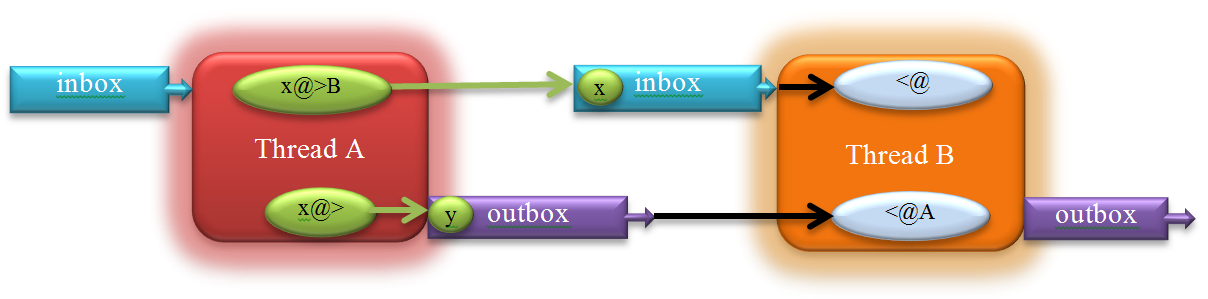
\includegraphics[width=5.75in,height=1.45in]{ub-img/thread-fig1.png}
\end{center}
\vspace{-0.25cm}{\sffamily\bfseries Figure 8-1:}
{\sffamily Inboxes and Outboxes for Thread Communication.}


\subsection*{\texttt{send} and \texttt{receive} operators}

The \texttt{@>} (send) and \texttt{{<}@} (receive) operators communicate
messages containing arbitrary data between threads. The operators support
co-expressions as well, with the same semantics. The send operator has the
syntax

\iconcode{
x @>T
}

\noindent
where \texttt{x} can be any data type, including null, which is equivalent to omitting
it. \texttt{T} refers to a thread to which \texttt{x} is transmitted: \texttt{x}
is placed in \texttt{T}'s inbox.  \texttt{x} can be picked by \texttt{T} using
the receive operator which is presented later.
\texttt{x @> \&main} may be used to send a message to the main thread.
The send operator can also have no destination, as in

\iconcode{
x @>
}

In this case \texttt{x} is sent to no one, instead it is placed in the sender's
outbox. The operator can be read as ``produce \texttt{x}''.  \texttt{x} can then
be picked up later by any thread wanting a value from this sender.  For example
the sender in this case might be a creating prime numbers and placing them in
its outbox to be ready for other threads.

The receive operator is symmetric to send, and takes two forms, with explicit
source or with no source, as follows:

\iconcode{
{<}@T \\
{<}@
}

\noindent
The first case reads ``receive a value from \texttt{T}''; it obtains a value
from \texttt{T}'s outbox. In the prime number example mentioned
above, \texttt{<@T} would be the way to get a prime number produced by
\texttt{T}. \texttt{{<}@} on the other hand reads values directly from the
receiver's inbox.  It reads messages sent explicitly to the thread doing the
receive operation.

Both \texttt{@>} and \texttt{{<}@} can succeed or fail. In the case of
\texttt{{<}@} the operator succeeds and returns a value from the corresponding
queue (inbox/outbox) depending on the operand if the queue is not empty. If the
queue is empty the operation fails directly. In the case of \texttt{@>}, if the
value is placed in the corresponding queue the operation succeeds and returns
the size of the queue. If the queue is full, the send operation fails. The
inbox/outbox for each thread is initialized to have a limited size (it can hold
up to 1024 values by default). This limit can be increased or decreased
depending on the application needs. The limits are useful so that queue sizes do
not explode quickly by default. They also provide an implicit
communication/synchronization as explained later in following sections.  Let us
look at the producer/consumer example again written using the new operators:

\iconcode{
procedure main() \\
\ \ \ p := thread produce() \\
\ \ \ c := thread consume(p) \\
\ \ \ every wait(p {\textbar} c) \\
end \\
\ \\
procedure produce() \\
\ \ \ every !10 @> \ \ \# place values in my outbox \\
end \\
\ \\
procedure consume(p) \\
\ \ \ i := 0 \\
\ \ \ while i {<} 10 do \\
\ \ \ \ \ \ if x := {<}@ p then\ \ \# get values from p \\
\ \ \ \ \ \ \ \ \ i +:= 1 \& write(x) \\
end
}

Each thread has exactly one inbox and one outbox, and each operator call is
mapped to only one of these inboxes or outboxes as seen in Figure 1.  All
messages from all threads coming to thread B in the figure end up in its
inbox. All threads trying to receive messages from A compete on A's outbox. Both
the inbox and the outbox queues are public communications channels, and it is
impossible to distinguish the source of a message if there are several threads
sending messages to the same thread at the same time. Furthermore, if
\texttt{{<}@} has an explicit source like A in Figure 1, it only looks in A's
outbox, and does not see messages from A coming directly to the
inbox. Applications that require the sender's address can attach that
information to messages by building them as records with two fields, one field
for data and the other containing the sender's address. A better approach for
private communications for some applications is the use of lists shared between
the two communicating threads or the use of private communication channels
discussed later in this document.


\subsection*{Inbox/Outbox and the \texttt{Attrib()} function}

As seen in previous sections, communication between threads is done though
inbox/outbox queues which have size limits. The size limit, which defaults to
1024, and the actual size dictate how synchronization is merged with the
communication. The size operator \texttt{*} can be used with a thread to query
its actual outbox size (how many values it contains, not the maximum limit), as
follows:

\iconcode{
outbox\_size := *T
}

But this is only a single attribute for one queue.  To access or change other
queue attributes, a new function \texttt{Attrib()} is introduced.  This function
uses the form \texttt{Attrib(handle, attribcode, value, attribcode, value,
  ...)}. The integer codes used by this function are defined in an include file
\texttt{threadh.icn}. This header file is part of the \texttt{threads} package,
which can be used by a program via

\iconcode{
import threads
}

When values are omitted, \texttt{Attrib()} generally returns attribute
values. To get the size of the outbox (the same as the \texttt{*} operator), the
code is

\iconcode{
outbox\_size := Attrib(T, OUTBOX\_SIZE)
}

\noindent similarly, 

\iconcode{
inbox\_size := Attrib(T, INBOX\_SIZE)
}

\noindent
gets the current size of the inbox. On the other hand

\iconcode{
Attrib(T, INBOX\_LIMIT, 64, OUTBOX\_LIMIT, 32)
}
sets the inbox and outbox size limits to 64 and 32 respectively. The following
table summarizes the available attributes and their meanings.

%% [DPW] For some reason, known only to itself, LaTeX insists on a page break
%% here and leaves about 90% of the preceding page blank.  I changed from
%% supertabular to tabular and the problem went away.
%% \begin{flushleft}
%% \tablehead{}
%% \begin{supertabular}{m{2.0941598in}m{1.9087598in}m{1.9108598in}}
%% Attribute &
%% Meaning &
%% Read/Write?\\
%% INBOX\_SIZE &
%% Number of items in the inbox &
%% Read Only\\
%% OUTBOX\_SIZE &
%% Number of items in the outbox &
%% Read Only\\
%% INBOX\_LIMIT &
%% The maximum number of items allowed in the inbox &
%% Read/Write\\
%% OUTBOX\_LIMIT &
%% The maximum number of items allowed in the outbox &
%% Read/Write\\
%% \end{supertabular}
%% \end{flushleft}

\begin{flushleft}
\begin{tabular}{p{1.6in} p{2.8in} p{1.5in}}
 Attribute & Meaning & Read/Write?\\
\hline
INBOX\_SIZE &
Number of items in the inbox &
Read Only\\
OUTBOX\_SIZE &
Number of items in the outbox &
Read Only\\
INBOX\_LIMIT &
The maximum number of items allowed in the inbox &
Read/Write\\
OUTBOX\_LIMIT &
The maximum number of items allowed in the outbox &
Read/Write\\
\end{tabular}
\end{flushleft}

\subsection*{Blocking send and receive}

In many situations senders and receivers generate and consume messages at
different speeds or based on needs. Instead of overloading slow receivers or
busy waiting for slow senders, the two ends of the communication need a
synchronizing mechanism to tell them when to send new messages or when a new
message is available. Two more send and receive operators provide such
functionality, the blocking send operator \texttt{@>{}>} and the blocking
receive operator \texttt{<{}<@}.  These can be used in the same way as
\texttt{@>} and \texttt{{<}@}, except that instead of failing when the operation
cannot be completed, the new operators block and wait until the operation
succeeds. In the simple producer/consumer example, the producer is only
producing 10 values, since the default size of the queue is 1024, using a
blocking send would not make any difference. The consumer however, can make use
of the blocking receive instead of spinning in some cases while the queue is
empty and the original blocking receive just keeps failing.  Take a closer look
at the consumer code again:

\iconcode{
procedure consume(p) \\
\ \ \ i := 0 \\
\ \ \ while i {<} 10 \ do \\
\ \ \ \ \ \ if x := {<}@ p then\ \ \# get values from p \\
\ \ \ \ \ \ \ \ \ i +:= 1 \& write(x) \\
end
}

Using an \texttt{if} statement with \texttt{{<}@} checks whether the operation
succeeds in receiving a value. A blocking receive is more suitable in this case
and it simplifies the loop slightly, since the \texttt{if} can be dropped, and
also the counter is not necessary anymore. The counter was previously necessary
because the loop needs to keep track of how many \texttt{{<}@} were needed to
count to 10. The consumer can be rewritten as

\iconcode{
procedure consume(p) \\
\ \ \# get exactly 10 values from p, block if necessary\\
\ \ \ every !10 do write({<}{<}@ p) \\
end
}

In some cases, a thread might want to use a blocking receive to get values from
a second thread, but it is not willing to block indefinitely; it may do some
other useful work instead of waiting. The \texttt{<{}<@} operator accepts a
timeout parameter to impose a limit on how long to wait for a result before
giving up. Here is how \texttt{<{}<@} would look in this case:

\iconcode{
result := timeout {<}{<}@ \ \ \ \ \# \ get from my inbox
}

or 

\iconcode{
result := timeout {<}{<}@ T\ \ \ \ \# get from T's outbox
}

The timeout operand is a non-negative integer denoting the maximum time to wait
in milliseconds.  Negative integers are treated as a null value, defaulting to
an indefinite blocking receive.  A 0 operand indicates no waiting time,
effectively resulting in a non-blocking receive.  The following table summarizes
the different forms of the send and receive operators and their operands:


\bigskip

\begin{flushleft}
\tablehead{}
\begin{supertabular}{m{0.8920598in}m{0.8643598in}m{4.10186in}}
\centering Operator &
\centering Operands &
\centering\arraybslash Behavior\\
\centering @>\par
\centering (send) &
\centering msg@> &
Place msg in my outbox, fail if the outbox is full\\
 &
\centering msg@>T &
Place msg in T's inbox, fail if T's inbox is full\\
\centering {<}@\par

\centering (receive) &
\centering {<}@ &
get a message from my inbox, fail if the inbox is empty\\
 &
\centering {<}@T &
get a message from T's outbox, fail if T's outbox is empty\\
\centering @{>}{>}\par

\centering (blocking send) &
\centering msg@{>}{>} &
Place msg in my outbox, block if the outbox is full\\
 &
\centering msg@{>}{>}T &
Place msg in my T's inbox, block if the T's inbox is full\\
\centering {<}{<}@\par

\centering (blocking receive) &
\centering {<}{<}@ &
Get a message from my inbox, block if the inbox is empty\\
 &
\centering {<}{<}@T &
Get a message from T's outbox, block if
it is empty\\
 &
\centering n{<}{<}@ &
Get a message from my inbox, block up to n milliseconds
waiting for an inbox message to become available\\
 &
\centering n{<}{<}@T &
Get a message from T's outbox, block up to n
milliseconds waiting for a message to become available there\\
\end{supertabular}
\end{flushleft}

\bigskip

Most applications use only a few of these modes. In a fast sender/slow receiver
application, the sender would block when the queue is full and unblock when the
queue is empty (using \texttt{@>{}>}). The receiver would consume messages from
the queue until it is empty, and then block until there is a new message added
to the queue (\texttt{<{}<@}). For some applications however this communication
scheme might not be optimal, hence many options are provided. The different
options in the table above give the programmer a wide range of control over when
to block or resume a thread based on the availability of data in the
communication queues. This control covers the needs of many applications and
provides simple ways to abstract concurrent programming activities such as load
balancing and efficient use of resources.

\subsection*{Private communication channels}

As mentioned in the previous sections, inbox and outbox communication queues are
visible by all threads all the time. In some scenarios two or more threads need
to communicate with each other without worrying about other threads sending and
receiving messages at the same shared queues. While it is possible to build a
protocol at the application level on top of the inbox and outbox queues to
achieve such behavior, it is simpler and more efficient to have the threads
communicate privately. This kind of communication can be done by sharing a list
between two threads and protecting it by an explicit mutex, or using a
thread-safe list. A more formal way for such communication is to use the
\texttt{channel()} function.

Starting a private communication is similar to a network connection, except that
this connection is taking place between two threads in the same process instead
of two different processes that may be on different machines. A private
communication channel between two threads can be created using the library
procedure \texttt{channel()}.

\texttt{channel()} is part of the \texttt{threads} package, so \texttt{import
  threads} is necessary to use it.  It takes one parameter, which is the thread
with which the connection will be initiated.  If \texttt{channel()} succeeds, it
returns a list representing a communication channel between the two
threads. Representing a bidirectional channel that can be used by the two
threads, given that each thread calls the function \texttt{channel()} with the
other thread as an argument.  Here is an example.

In thread A:

\iconcode{
\ \ \ \ \ \ \ \ chB := channel(B) \ {\textbar} "failed to open a channel with B"
}

In thread B:

\iconcode{
\ \ \ \ \ \ \ \ chA := channel(A) \ {\textbar} "failed to open a channel with A"
}

A channel is a \emph{directional} communication medium.  One thread should use
it as an outbox, and the other should use it as an inbox; only one thread will
send messages over the channel while the other receives them from the other
end. The provided channel can be used with the communication operators (all four
of them) with the same semantics as before. The only difference in this case is
that the right operand is a communication channel instead of a thread.  In the
channel example below, the main thread transmits the consumer's identity to the
producer (\texttt{c @> p}), who receives it via \texttt{c := <{}<@}:

\iconcode{
import threads \\
procedure main() \\
\ \ \ p := thread produce() \\
\ \ \ c := thread consume(p) \\
\ \ \ c @> p \\
\ \ \ every wait(p {\textbar} c) \\
end \\
\ \\
procedure produce() \\
\ \ \ c := {<}{<}@ \\
\ \ \ chC := channel(c) \\
\ \ \ every !10 @> chC \ \ \# place values in channel c \\
end \\
\ \\
procedure consume(p) \\
\ \ \ chP := channel(p) \\
\ \ \ every !10 do write({<}{<}@chP) \\
end
}

\subsection*{A simple thread pool}
In some cases the explicit creation of a thread for each concurrent activity is
the simplest and most transparent way of writing the program, especially if the
threads need access to the local variables of the procedure that created them.
In other cases the work can be more expeditiously carried out by a pool of
``worker'' threads, which execute tasks that are handed to them.  The threads
package contains a simple thread pool that may be used for this purpose: it has
four procedures.

\bigskip\hrule\vspace{0.1cm}
\noindent\makebox[1.5in][l]{\texttt{MakePool(n)}\vspace{0.75in}}
Create a pool of \texttt{n} worker threads. The default value for \texttt{n} is
2 + the number of processors reported in \texttt{\&features}.There is usually
not much to be gained by having many more active threads than the number of
available processors (unless a significant number are idle, waiting for an event
to happen).

\bigskip\hrule\vspace{0.1cm}
\noindent\makebox[2.5in][l]{\texttt{Dispatch(proc, params, ...)}\vspace{0.75in}}
Queue a task to be executed by a thread from the pool. If a thread is available
the procedure will be called immediately with the supplied parameters, otherwise
it will be called when a thread becomes available.\\

\bigskip\hrule\vspace{0.1cm}
\noindent\makebox[1in][l]{\texttt{isIdle()}\vspace{0.75in}}
Succeeds if no worker threads are active and there are no tasks in the queue.\\

\bigskip\hrule\vspace{0.1cm}
\noindent\makebox[1.5in][l]{\texttt{ClosePool()}\vspace{0.75in}}
Shuts down the pool after remaining tasks have finished
(including those that are in the queue). \texttt{ClosePool} does not return
until the pool has been shut down and all the threads have finished, which
provides a simple way of synchronizing the concurrent activities with the
controller thread (often \texttt{\&main}).\\

Although waiting for everything to finish is the most usual (and safest)
technique, if waiting is not required a simple way to achieve it is to write
{\small
\iconcode{
\>thread\{ClosePool()\}
}
}
Note that calling \texttt{ClosePool} directly in a worker thread will lead to
deadlock (because the thread will be waiting for itself to terminate).  The same
thing happens if you write \texttt{Dispatch(ClosePool)}.  There is some risk
attached to not waiting for the pool to complete its work because if the main
thread terminates the whole program finishes --- regardless of the state of the
thread pool.

The thread pool is minimalist by design. There are a number of extra facilities
that could, perhaps, be added --- cancellation of a task, place a task at the
front of the queue, rather than the rear --- but these are left as an exercise
for the reader who needs them.

\section{Practical examples using threads and messages}
This section starts with a discussion of an early version of a program that
forms part of an indexing system for \LaTeX\ files, which are the source for a
book.  The system operates in three phases:
\begin{enumerate}
\item An analysis phase, where the possible words to be indexed are gathered
      from the source files.
\item A manual review phase to select the index terms. Good indexing
      is an art and some judgement must be exercised when choosing
      what to index and how to refer to it.
\item An insertion phase where the chosen terms are located and the indexing
      terms inserted into the source files.
\end{enumerate}
We focus on the first (analysis) phase. Here the files are read in and every
``word'' is put into a table that counts how many times that word occurs. 
Words that occur too many times (either in an individual source file, or the
document as a whole) are rejected as indexing candidates because they are likely
to be the common words that are of no value in an index.
A simple program to analyze the files is something like the following. It uses
three nested loops to read each file, split every line into words and put the
results into a file table. At the end of each file, it copies eligible words from
the file table into the document table.
Two parameters, \texttt{perFile} and \texttt{perDoc}, govern the limits that cause
a particular word to be rejected as an index candidate. \texttt{perDoc} is used
in the \texttt{reportWords} procedure, which is not shown.

{\small
\iconcode{
global perFile\ \ \ \ \# If a wordcount exceeds this in a single tex file it is rejected\\
global perDoc\ \ \ \ \# If a wordcount exceeds this in the whole document it is rejected\\
\\
procedure main(args)\\
\>local nFiles\\
\>local f, wt, dt, word, texWord, fileName, line, count, x\\
\\
\>\# argument and option processing omitted for clarity\\
\\
\>dt := table(0)\\
\>texWord := \&letters ++ "\_-{\textbackslash}'"\\
\>count := 0\\
\\
\>every fileName := !args do \{\\
\>\>if f := open(fileName, "r") then \{\\
\>\>\>wt := table(0)\\
\>\>\>every line := !f do \{ \# put each word in the word table\\
\>\>\>\>line ? \{while tab(upto(texWord))\\ 
\>\>\>\>\>\do \{word := tab(many(texWord)); wt[word] +:= 1; count +:=1 \}\\
\>\>\>\>\>\}\\
\>\>\>\}\\
\\
\>\>\>\# Add the candidate words used in this file to the master table.\\
\>\>\>every word := key(wt) do if (x := wt[word]) <= perFile then dt[word] +:= x\\
\>\>\>close(f)\\
\>\>\} else \{write(\&errout, "Cannot open ", fileName) \}\\
\>\}\\
\>reportWords(dt)\\
\\
\>return\ \ \# Success\\
end
}
}

Whilst this program works, albeit with an idiosyncratic definition of what
constitutes a word, it suffers from a serious defect: it only analyzes one file
at a time so a large proportion of the available processing power is unused (on
the author's machine, which reports 8 cores, the figure works out at 87.5\% idle).
We can do {\em much} better than that.

In the following version, which uses the \texttt{threads} library package, each
file is processed in parallel by a separate thread drawn from a pool of worker threads. 
After the analysis of each file is complete, the results are sent to a separate
``accumulator'' thread that aggregates the results.

\bigskip
{\small
\iconcode{
import threads\\
global perFile\ \ \ \ \# If a wordcount exceeds this in a single tex file it is rejected\\
global perDoc\ \ \ \ \# If a wordcount exceeds this in the whole document it is rejected\\
global countingThread\\
\\
procedure main(args)\\
\>local nFiles\\
\\
\>\# argument and option processing omitted for clarity\\
\\
\>nFiles := *args\\
\>MakePool() \# no parameter means default of 2 + no. of processors\\
\\
\>\# Start a "counting thread" to accumulate answers from the analysis threads.\\
\>Dispatch(accumulator)\\
\\
\>\# Analyze each file in a separate thread. Send the results to the accumulator.\\
\>every Dispatch(analyze, !args)\\
\\  
\>waitFor(nFiles)             \# Wait for all files to be analyzed.\\
\\
\>\# Since all the analyzers have now finished, it is safe to end the counting thread.\\
\>\# It will get all the answers that have previously been sent before receiving "end".\\
\>"end" @{>}{>} countingThread\\
\\
\>ClosePool()                 \# ClosePool returns when all threads have finished.\\
\\
\>return  \# Success\\
end
}
}

The procedures called by main (except for \texttt{waitFor}) are all pretty much
the same as the corresponding lines of code in the preceding example. Each
analysis thread sends a message to the main thread when it has finished.  Since
the main thread knows how many files there are to be processed, it can wait
until every file has been analyzed.
{\small
\iconcode{
\# Wait for the specified number of messages before returning\\
procedure waitFor(messages :integer)\\
\>repeat \{ {<}{<}@ ; if 0 >= (messages -:= 1) then return \}\\
end
}
}

The \texttt{analyze} procedure is the same as the previous example, except that
it sends a result to the accumulator thread and a ``finished'' message to the
main thread.
{\small
\iconcode{
procedure analyze(fileName :string)\\
\>local f, line, count := 0, word, wt := table(0)\\
\>local texWord := \&letters ++ "\_-{\textbackslash}'"\\
\>if f := open(fileName, "r") then \{\\
\\
\>\>every line := !f do \{ \# put each word in the word table\\
\>\>\>line ? \{while tab(upto(texWord)) do \{\\
\>\>\>\>\>word := tab(many(texWord)); wt[word] +:= 1; count +:=1 \}\\
\>\>\>\}\\
\>\>\}\\
\>\>wt @{>}{>} countingThread   \# Send the words to the accumulator thread\\
\>\>close(f)\\
\>\} else \{ write(\&errout, "Cannot open ", fileName) \}\\
\\
\>"end" @{>} \&main   \# Tell the main thread that a file has been analyzed\\
\>return \# success\\
end
}
}

The accumulator thread gets messages from the analysis threads and from the main
thread. It uses the type of the message to distinguish between them. Before
starting, it writes its thread id to a global variable so other threads know
where to send messages. 
{\small
\iconcode{
procedure accumulator()\\
\>local msg, word, x, dt := table(0)\\
\>\# publish the thread Id so other threads can send messages.\\
\>countingThread := \&current\\
\>repeat \{\\
\>\>msg := {<}{<}@\\
\>\>case type(msg) of \{\\
\>\>\>"table" :  \# Add the candidate words in this file to the master table.\\
\>\>\>\>\{ every word := key(msg)\\
\>\>\>\>\>do if (x := msg[word]) <= perFile then dt[word] +:= x \}\\
\>\>\>"string" : \# Final message from the main thread.\\
\>\>\>\>\{ reportWords(dt); return \}\\
\>\>\>default: stop("Invalid message sent to counting thread")\\
\>\>\}\\
\>\}\\
end
}
}

Note: this design has a race condition --- it is possible that an analysis
thread that has started {\em after} the accumulator could finish its analysis
{\em before} the accumulator has even started. In that case the program would
terminate because of an attempt to send a message to \texttt{\&null}: it has
never happened, but the behaviour is theoretically possible (and a correct
concurrent program may make {\em no} assumptions about timing). One cure would
be for the main program to wait for a message from the accumulator thread before
starting the others. A less elegant solution would be to delay until the
\texttt{countingThread} variable is not null.

Although the tables themselves may be quite large, because a table is a mutable
type it is passed by reference, so the messages passed between threads are quite
small. Extra work has to be done to pass messages and to coordinate the threads
but the savings outweigh the extra work by a considerable margin. The graph
below plots the run times of the original sequential program and the concurrent
program using a different number of threads to perform the analysis.

\begin{figure}[h]
{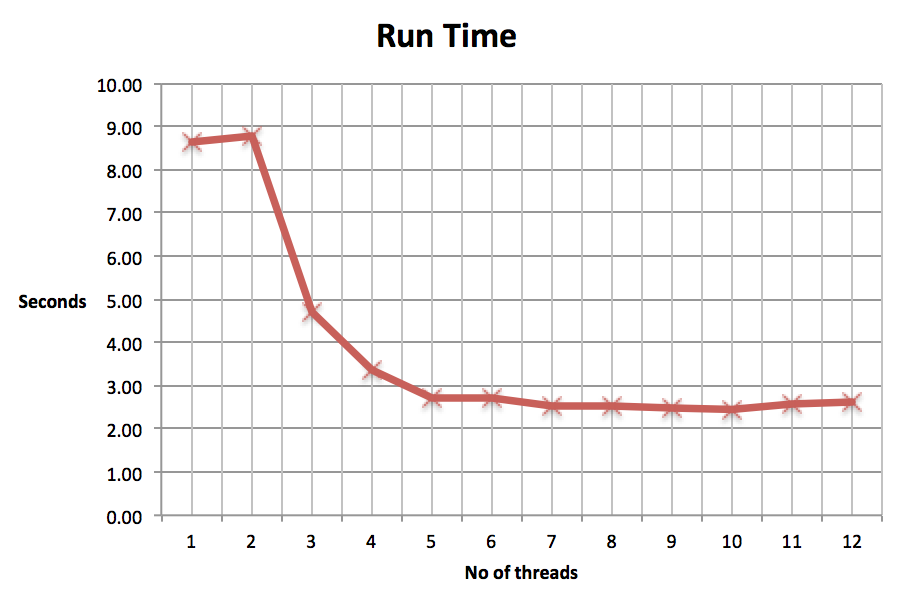
\includegraphics[scale=0.75]{ub-img/threadPerformance.png}}
\end{figure}

Because of the accumulator thread, the number of threads performing
the analysis is one less than the graph shows. This explains the
slight ``bump'' at two threads: there is only one analysis thread, so
we get the performance of the sequential version {\bf plus} the
overheads of message passing. With two analysis threads (three in
total) the run time is halved and with four analysis threads the
performance is roughly quadrupled. Adding more threads doesn't really
increase the performance in this particular example (the test machine
reports eight processors but it's really four dual hyper-threaded cores: the
lack of speed-up after four analysis threads suggests that the dual
hyper-threads don't have quite as much ``grunt'' as two separate cores)

There is no explicit synchronization because the analysis threads are not
contending with each other --- if the table that counted words in the whole
document were global and each analysis thread added it's own results to the
global table then contention for the table might be a performance bottleneck ---
instead, the analysis threads are just passing their results in a message and
getting on with their day. An accumulator, for the price of an extra
thread, can often result in a worthwhile increase in performance.

This design pattern (process in parallel and send results to a single
accumulator) can be used in many different circumstances and, in most cases, the
reduction in contention more than makes up for the cost of the extra
thread. 

\bigskip

\subsection{Disk space usage}
The unix \texttt{du} utility can be used to traverse a filesystem and report on
the space used.  If, instead of a recursive traversal of each directory, the
separate directories are analyzed in parallel and the results sent to an
accumulator the result is usually faster. The process may be initiated by a
procedure like the following
{\small
\iconcode{
\# Analyze a directory and wait until the analysis is finished\\
procedure analyze(path)\\
\>local thisThread := \&current\\
\>MakePool()\\
\>Adder := thread \{ Dispatch(du, ({\textbackslash}path | "." )); GatherResults() @{>}{>} thisThread \}\\
\>write("total size = ", {<}{<}@ )\\
\>ClosePool()\\
\>return \# success\\
end
}
}
Note that instead of using a thread from the pool as an accumulator, one is
created on the fly (this is another way of avoiding the start-up race discussed
in the previous example). The \texttt{du} procedure analyzes a directory, adding
up the size for regular files, ignoring special files and handing off (sub)
directories to another thread. At the end it sends off the total for that
directory (but not it's children) to the accumulator thread.

Before analyzing a directory, it also sends off a message to the accumulator
announcing its intent. The reasons for this are discussed later.  In the interests
of clarity, some code dealing with loops in the filesystem has been omitted.
{\small
\iconcode{
\# Get the disk usage for a directory. Do sub-dirs in parallel with this one.\\
procedure du(d, parent)\\
\>local st, fd, f, path, kb := 0\\
\\
\>fd := open(d) | \{ Report("Cannot open", d); return \}\\
\>\# send a "starting analysis of d" message to the Adder\\
\>[d, \&null] @{>}{>}Adder\\
\\
\>while f := !fd do \{ \\
\>\>if f == ("." | "..") then next\\
\\
\>\>if st := stat(path := d || "/" || f) then \{\\
\>\>\>case st.mode[1] of \{\\
\>\>\>\>"-": \# Normal file - add its rounded size to the total for this directory\\
\>\>\>\>\>kb +:= ((st.size {<} st.blksize) |\\
\>\>\>\>\>\>\>\>st.blksize * ceil(st.size/(0.0 + st.blksize)))/1024\\
\\
\>\>\>\>"d": \# Directory - hand it off to a worker thread to analyze in parallel\\
\>\>\>\>\>Dispatch(du, path, d, f)\\
\\
\>\>\>\>"l" | "s" | "b" | "c" | "p" | "|": \# Ignore special files, symbolic links, pipes etc.\\
\>\>\>\>next\\
\\
\>\>\>\>default: Report("Cannot handle mode \"", st.mode, "\", file ", path)\\
\>\>\>\}\\
\>\>\} else \{\\
\>\>\>Report("Cannot stat", path)\\
\>\>\}\\
\>\}\\
\\
\>close(fd)\\
\>[d, kb,] @{>}{>} Adder   \# Send the result from analysis of d to the Adder\\
end
}
}

The Adder thread, which calls procedure \texttt{GatherResults}, gets results for
each directory until it's all over. Each directory results in two messages:
\texttt{[d, null]} followed, a little later by \texttt{[d, size]}.  Results for
child directories of \texttt{d} might come {\em before} the second message, but
will never precede the first.

{\small
\iconcode{
procedure GatherResults()\\
\>local msg, kb := 0\\
\\
\>repeat \{ \\
\>\>msg := {<}{<}@; kb +:= {\textbackslash}msg[2]\\
\\
\>\>\# Have we finished? The question is trickier than it looks!\\
\>\>if IsIdle() \& (Attrib(Adder,INBOX\_SIZE) = 0) then return kb\\
\>\}\\
end
}
}

Now to the discussion of ``Have we finished?'' The reason the question is tricky
is because \texttt{GatherResults} operates in parallel with the analysis;
perhaps before it has even started.  We must ensure that we don't bail out
before at least one directory has been analyzed, which is achieved by placing
the test after the reception of the first message --- this is one of the reasons
for sending two messages per directory. We must check the analysis is finished
i.e. there is no work in progress.  The WIP logic depends on \texttt{du} queuing
new work {\em before} reporting the result of analyzing a directory. Finally, we
must have processed all of the messages.

Note that \texttt{IsIdle()} must be true before checking the message queue is
empty; otherwise, there is a race between the analysis thread and
\texttt{GatherResults} (We might see an empty message queue, then the analyzer
posts \texttt{[d, size]} and finishes before we call \texttt{IsIdle()}: The
result would be that we'd ignore the final message, or messages).

It is sometimes true that deciding when a concurrent algorithm has finished ---
without terminating prematurely or discarding some of the final results or never
terminating --- is harder than writing the processing algorithm itself!

The reader may be wondering why the directory name is passed to the
\texttt{GatherResults} procedure, which doesn't use it.  The reason is that
these examples are edited extracts from a larger program that builds a structure
that represents the directory and its child sub-directories. It then displays a
series of pie charts (one for each directory) showing where all the space has
gone.  It needs the directory names to label the segments of each pie chart. The
other reason for passing two messages per directory is that the full program
needs to set up the structure for a directory before receiving any results for
its children.

When analyzing a fairly large (500GB) directory, the pie chart program --- which
runs on the Unicon interpreter and is based on the code examples above ---
outperforms the built in \texttt{du} program by almost an order of magnitude on
an eight core processor; the built in program is presumably written in C and
optimised but, crucially, it is single threaded.

\subsection{More suggestions for parallel processing}
If several files are involved, it is often quite easy to see how the
processing may be done in parallel but there are other cases --- some more
obvious than others --- where it might prove useful:
\begin{description}
\item[Monte Carlo methods]
  Any problem that calls for a large number of trials, where the result
  of one trial does not affect subsequent trials is amenable to being
  written as a parallel application.
\item[Matrix multiplication]
  Large matrices may be multiplied in parallel, either by a naive rewrite of the
  sequential ($O(n^3)$) algorithm or by dividing the matrix up into blocks (divide
  and conquer) and handling each block in a separate thread.
\item[Unicon compiler]
  Analysis and code generation is largely independent for each Unicon
  procedure. It might be possible to farm out larger procedures to a thread pool
  and thereby increase the overall performance of the compiler.
\item[grep]
  If the regular expression is computationally expensive, spreading out the
  analysis work for each line of the file to a thread pool might be faster.
\end{description}
The last two  suggestions are speculative but demonstrate that the world can look
quite different when viewed through concurrent spectacles.




\section{Summary}

True concurrency opens up major new application domains for the Unicon language.
More importantly, it enables the language to utilize more than the small
fraction of modern processors utilized by traditional sequential execution. For
example, on a typical quad-core desktop, many applications will be able to get
between 2$\times$ and 4$\times$ the performance of a sequential Unicon program
with relatively minor changes. This is comparable to the speedup typically
delivered by the optimizing compiler.  Some applications will be able to do even
better on processors with more cores.

This document presented Unicon's concurrency facilities from a programmer's
perspective. The implementation and its performance are described in more detail
in [Al-G12]. There are major areas for future work, including GPU- and APU
support, and various forms of implicit concurrency that can be added to the
language.
